\subsubsection{Linear Regression}

In fact, the network architecture in figure \ref{fig:xorgatenetwork} uses one neuron to simulate an OR logic gate ($L_{1,1}$) and another neuron to simulate an AND logic gate ($L_{1,2}$). Seeing the logic of an \acrshort{xor} gate:

\begin{eqnarray}
    A \oplus B = (A \land \neg B) \lor (\neg A \land B) = (A \lor B) \land (\neg A \lor \neg B)
\end{eqnarray}

It makes sense to use the OR and AND gates in the network. You can see graphically how each neuron works in the following image:
\begin{figure}[H]
    \centering
    
\includegraphics[width=15cm]{images/state-of-art/regression/xor.png}
    \caption{OR($L_{1,1}$), AND($L_{1,2}$) y \acrshort{xor}($L_{2,1}$) logic gates}
    \label{fig:orandxorgraph}
\end{figure}

Each of these neurons is performing a sorting task, simply checking whether the input data is on one side of the line or the other. This is because the perception has been defined in such a way that it can only return $0$ or $1$. But eliminating that classification step that has been defined in equation \ref{eqn:perceptron}, would result in a linear regression such that:
\begin{eqnarray}
  y = w \cdot x + b
      \label{eqn:neuronsimple}
\end{eqnarray}

A linear regression is the other type of task that a neuron can solve. This is one of the main differences between modern neurons and perceptrons. Perceptrons are only programmed to perform one sorting task, but neurons can be programmed for other types of cases. Although as will be explained later, a perceptron is a type of neuron with a step activation function (see section \ref{activationfunction}).
\newline

\begin{figure}[H]
    \centering
    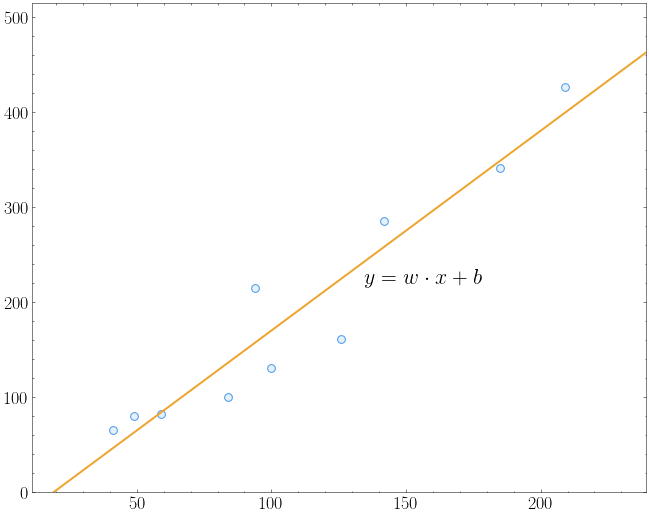
\includegraphics[width=9cm]{images/state-of-art/regression/regression.png}
    \caption{Example of linear regression in a two-dimensional space}
    \label{fig:regression}
\end{figure}

A linear regression is a method that studies the relationship between several variables and thus generates a model that can be used to estimate other values. Mathematically, in a multidimensional space $n$, a regression is defined as follows:


\begin{eqnarray}
  y = w_0 + w_1x_1 + w_2x_2 + ... + w_nx_n
  \label{linealregression}
\end{eqnarray}


In this equation there is an independent term $w_0$, and for each dimension, there will be a value $w$ and an $x$-value associated with it. Geometrically, in a space of two dimensions, $z$ will be a line, a plane if they are three dimensions and a hyperplane for greater than three dimensions, which cannot be represented graphically. In fact, it can be observed that equation \ref{eqn:neuronsimple} is the function of a line, being $b$  the independent term.
\newline

From this point onwards, $z$ will be used to refer to the linear regression that is calculated in a neuron:
\begin{equation}
  z \equiv y = w \cdot x + b
  \label{eqn:z_equation_init}
\end{equation}



